\documentclass[conference]{IEEEtran}
\IEEEoverridecommandlockouts

\usepackage{cite}
\usepackage{amsmath,amssymb,amsfonts}
\usepackage{graphicx}
\usepackage{textcomp}
\usepackage{xcolor}
\usepackage{booktabs}
\usepackage{multirow}
\usepackage{url}

\begin{document}

\title{Do Hand-Crafted Importance Maps Help Wavelet Image Compression?\\
A Controlled Study with the Missing Baselines}

\author{\IEEEauthorblockN{Abir Gupta}
\IEEEauthorblockA{\textit{Independent Researcher}\\
Bengaluru, India \\
abir.guptaaa@gmail.com}}

\maketitle

\begin{abstract}
For two decades, papers have proposed steering lossy image codecs with
hand-crafted perceptual importance maps built from edge, texture, and
saliency cues. Surveying twelve such works (2001--2023), we find that none
report the two controls needed to isolate the importance map's contribution:
a same-codec uniform-allocation baseline at matched bitrate, and sanity
controls with content-uncorrelated maps. We run both. Using a tile-based
JPEG 2000 pipeline on the Kodak dataset, we compare five importance
configurations against uniform tiling and single-pass JPEG 2000 across four
bitrates, evaluating global fidelity, fidelity restricted to the top-15\%
most-important regions, and LPIPS, with per-image bitrate-matched anchoring
and paired statistics. Three findings emerge. (1)~The tiling vehicle itself
costs $3.4$--$4.2$~dB versus single-pass encoding at matched bitrate
($p<0.001$). (2)~Importance maps do redirect fidelity as intended: relative
to uniform tiling, the multi-component map gains up to $+3.7$~dB inside
salient regions ($p<10^{-4}$)---but at a poor exchange rate, sacrificing
$2$--$7$~dB of background quality. (3)~The redirect never overcomes the
vehicle: single-pass JPEG 2000 outperforms every importance variant on every
metric \emph{including inside the salient regions the maps prioritize}
($3.3$--$14$~dB, $p<0.001$), while the maps cost $110\times$ the encoding
time. We conclude that post-hoc importance masks cannot compete with the
codec's own rate--distortion optimization; region-of-interest behavior must
be integrated into rate control, not bolted on.
\end{abstract}

\begin{IEEEkeywords}
Image compression, JPEG 2000, perceptual coding, saliency, region of interest, negative results
\end{IEEEkeywords}

\section{Introduction}

Human observers do not weight all image regions equally, so it is intuitive
that a codec should not either. This intuition has produced a steady stream
of importance-guided compression proposals: saliency-driven bit allocation
\cite{guo2010visual,barua2015saliency}, attention-weighted rate control
\cite{li2011visual,kaur2020regional}, ROI-prioritized coding
\cite{christopoulos2000jpeg,cai2017closed}, and multi-cue fusions of edges,
texture, and saliency.

Yet the experimental record has a hole. Table~\ref{tab:survey} summarizes
twelve importance-guided compression papers spanning 2001--2023. None runs a
\emph{content-uncorrelated sanity control} (a random or inverted importance
map), and ten of twelve never compare against \emph{their own codec with
uniform allocation at matched bitrate} on global fidelity; the remaining two
evaluate exclusively on attention-weighted or subjective scores, leaving the
global-fidelity cost unreported. Without these controls, reported gains
cannot be attributed to the importance model rather than to codec choice or
metric choice.

This paper supplies the missing controls. We build a deliberately simple
importance-guided pipeline---a multi-component map (edge + texture +
saliency) driving per-tile compression ratios in JPEG 2000---and evaluate it
the way the literature's claims demand: at matched bitrate, against uniform
allocation on the \emph{same} pipeline, against single-pass JPEG 2000,
inside and outside the regions the map marks as important, across four
bitrates, with paired statistics on 24 images.

We ask three questions. \textbf{Q1:} What does the implementation vehicle
(tile-based variable-rate coding) cost by itself? \textbf{Q2:} Do importance
maps actually redirect fidelity toward important regions, as claimed?
\textbf{Q3:} Is the net effect ever positive against the codec's own
allocation? The answers---quantified in
Section~\ref{sec:results}---are: a lot ($3.4$--$4.2$~dB), yes (up to
$+3.7$~dB in salient regions versus uniform tiling), and no (single-pass
JPEG 2000 wins everywhere, even inside the salient regions).

We frame the study honestly: JPEG 2000's encoder already performs
post-compression rate--distortion optimization (PCRD-opt)
\cite{taubman2002jpeg2000}, which allocates bits near-optimally for MSE at a
given rate. Overriding an MSE-optimal allocator with a heuristic cannot
improve global PSNR---that much is theory. What theory does \emph{not}
predict, and what we measure, is (a)~the size of the penalty, (b)~whether
the promised foreground gains materialize and at what background cost, and
(c)~whether perceptual metrics (LPIPS) tell a different story than PSNR.

\section{Related Work}

\begin{table*}[t]
\caption{Twelve importance-guided compression papers and the controls they report.
``Uniform ctrl'': same-codec uniform-allocation baseline at matched bitrate,
evaluated on global fidelity. ``Sanity ctrl'': random or inverted importance map.
``Fusion abl.'': ablation of individual importance components.}
\label{tab:survey}
\begin{center}
\small
\begin{tabular}{llllccc}
\toprule
\textbf{Paper} & \textbf{Importance model} & \textbf{Codec} & \textbf{Primary metric} & \textbf{Uniform ctrl} & \textbf{Sanity ctrl} & \textbf{Fusion abl.} \\
\midrule
Ouerhani et al. 2001 \cite{ouerhani2001adaptive} & Itti--Koch saliency & custom DCT & subjective, ROI quality & no & no & --- \\
Christopoulos et al. 2000 \cite{christopoulos2000jpeg} & manual ROI mask & JPEG 2000 & ROI PSNR & n/a & no & --- \\
Guo \& Zhang 2010 \cite{guo2010visual} & phase-spectrum saliency & custom multires. & subjective, ratio & no & no & --- \\
Li et al. 2011 \cite{li2011visual} & Itti attention & H.264 & eye-tracking-weighted PSNR & partial$^{\dagger}$ & no & --- \\
Barua et al. 2015 \cite{barua2015saliency} & GBVS-style saliency & wavelet/SPIHT & low-rate ROI quality & no & no & --- \\
Cai et al. 2017 \cite{cai2017closed} & graph saliency & JPEG & ROI/non-ROI trade-off & no & no & --- \\
Prakash et al. 2017 \cite{prakash2017msroi} & CNN multi-structure & JPEG & subjective, per-region & no & no & no \\
Z\"und et al. 2013 \cite{zund2013content} & saliency + retargeting & JPEG & subjective & no & no & --- \\
Zhang et al. 2021 \cite{zhang2021attention} & learned saliency skeleton & learned codec & RD, subjective & no & no & no \\
Kaur et al. 2020 \cite{kaur2020regional} & attention + sensitivity & HEVC & subjective & partial$^{\dagger}$ & no & no \\
ROI-Swin 2023 \cite{roiswin2023} & learned ROI & learned codec & ROI-weighted RD & no & no & no \\
This work & edge+texture+saliency & JPEG 2000 & global + region PSNR, SSIM, LPIPS & \textbf{yes} & \textbf{yes} & \textbf{yes} \\
\bottomrule
\end{tabular}
\end{center}
{\footnotesize $^{\dagger}$Standard encoder at matched rate, but evaluated only on
attention-weighted or subjective metrics; global-fidelity cost unreported.}
\end{table*}

\textbf{Perceptual importance for compression.} Saliency-guided methods
\cite{guo2010visual,barua2015saliency} allocate bits to attention-grabbing
regions; JND models \cite{wu2017just} bound quantization noise below
visibility thresholds; attention-weighted rate control has been applied to
video \cite{li2011visual,kaur2020regional}. The strongest claims in this
literature concern subjective or attention-weighted quality, not global
PSNR. Our region-restricted PSNR and LPIPS measurements are designed to
evaluate exactly that claim objectively.

\textbf{JPEG 2000 rate control.} JPEG 2000 \cite{taubman2002jpeg2000}
couples a wavelet transform with EBCOT and PCRD-opt rate allocation, which
distributes bits across code-blocks to minimize distortion at the target
rate. The standard's Maxshift and scaling-based ROI modes
\cite{christopoulos2000jpeg} integrate region priorities \emph{inside} this
machinery. The pipelines surveyed above instead overlay importance
externally---the design we test.

\section{Experimental Design}

\subsection{Importance maps}
We fuse three classical cues,
$\mathcal{I} = \alpha \mathcal{E} + \beta \mathcal{T} + \gamma \mathcal{S}$:
Canny edge strength $\mathcal{E}$ (Gaussian-smoothed, $\sigma{=}2$), local
FFT texture energy $\mathcal{T}$ ($16{\times}16$ windows), and spectral
residual saliency $\mathcal{S}$ \cite{hou2007saliency}, each normalized to
$[0,1]$ (visualized in Fig.~\ref{fig:importance_maps}). Configurations
tested: \textbf{default} $(0.4,0.3,0.3)$, \textbf{edge-only},
\textbf{texture-only}, \textbf{saliency-only}, \textbf{equal}
$(1/3,1/3,1/3)$, and \textbf{uniform} (constant map; every tile receives the
base ratio---the null allocation).

\begin{figure}[t]
\centering
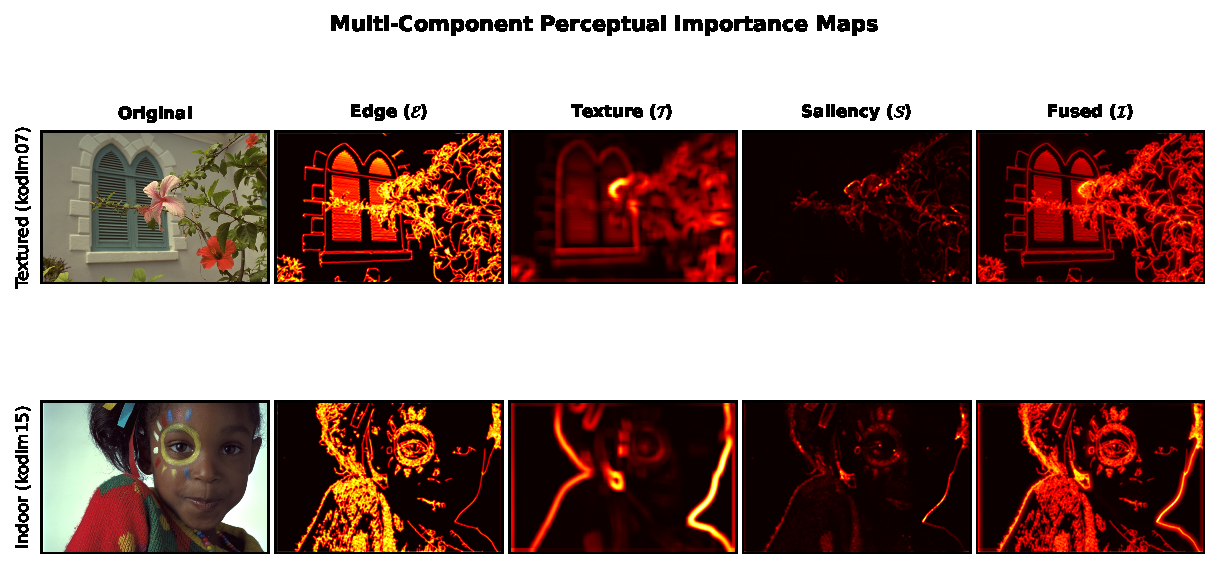
\includegraphics[width=\columnwidth]{figures/importance_maps.pdf}
\caption{Importance components and fusion for two Kodak images. From left:
original, edge $\mathcal{E}$, texture $\mathcal{T}$, saliency $\mathcal{S}$,
fused $\mathcal{I}$.}
\label{fig:importance_maps}
\end{figure}

\subsection{Pipeline and baselines}
Images are split into $64{\times}64$ tiles; each tile is JPEG 2000-encoded
(OpenJPEG 2.5.2) at a compression ratio set by its mean importance
$\bar{\mathcal{I}}_t$: ratio $R/2$ if $\bar{\mathcal{I}}_t{>}0.30$, $R$ if
$\bar{\mathcal{I}}_t{>}0.15$, else $3R$ (capped at 60), for base ratios
$R \in \{8, 16, 30, 50\}$. The \textbf{uniform} variant assigns $R$ to every
tile, isolating the tiling vehicle's cost. The \textbf{single-pass} baseline
encodes the whole image conventionally at ratio $R$---the codec's own
PCRD-opt allocation, untouched.

\subsection{Evaluation protocol}
\textbf{Dataset:} Kodak (24 images, $768{\times}512$).
\textbf{Metrics:} PSNR, SSIM, LPIPS \cite{zhang2018lpips}, and PSNR
restricted to the top-15\% highest-importance pixels (mask derived from the
default map and \emph{fixed across all variants}) and to the bottom-40\%.
\textbf{Bitrate fairness:} because variants land at different bitrates for
the same $R$, every measurement is reported as a \emph{gap} against that
image's own single-pass RD curve interpolated at the measurement's exact
BPP. \textbf{Statistics:} one-sample $t$-tests on per-image gaps and paired
$t$-tests between variants ($n{=}24$); significance marked
$^{*}p{<}.05$, $^{**}p{<}.01$, $^{***}p{<}.001$.

\section{Results}\label{sec:results}

\begin{figure*}[t]
\centering
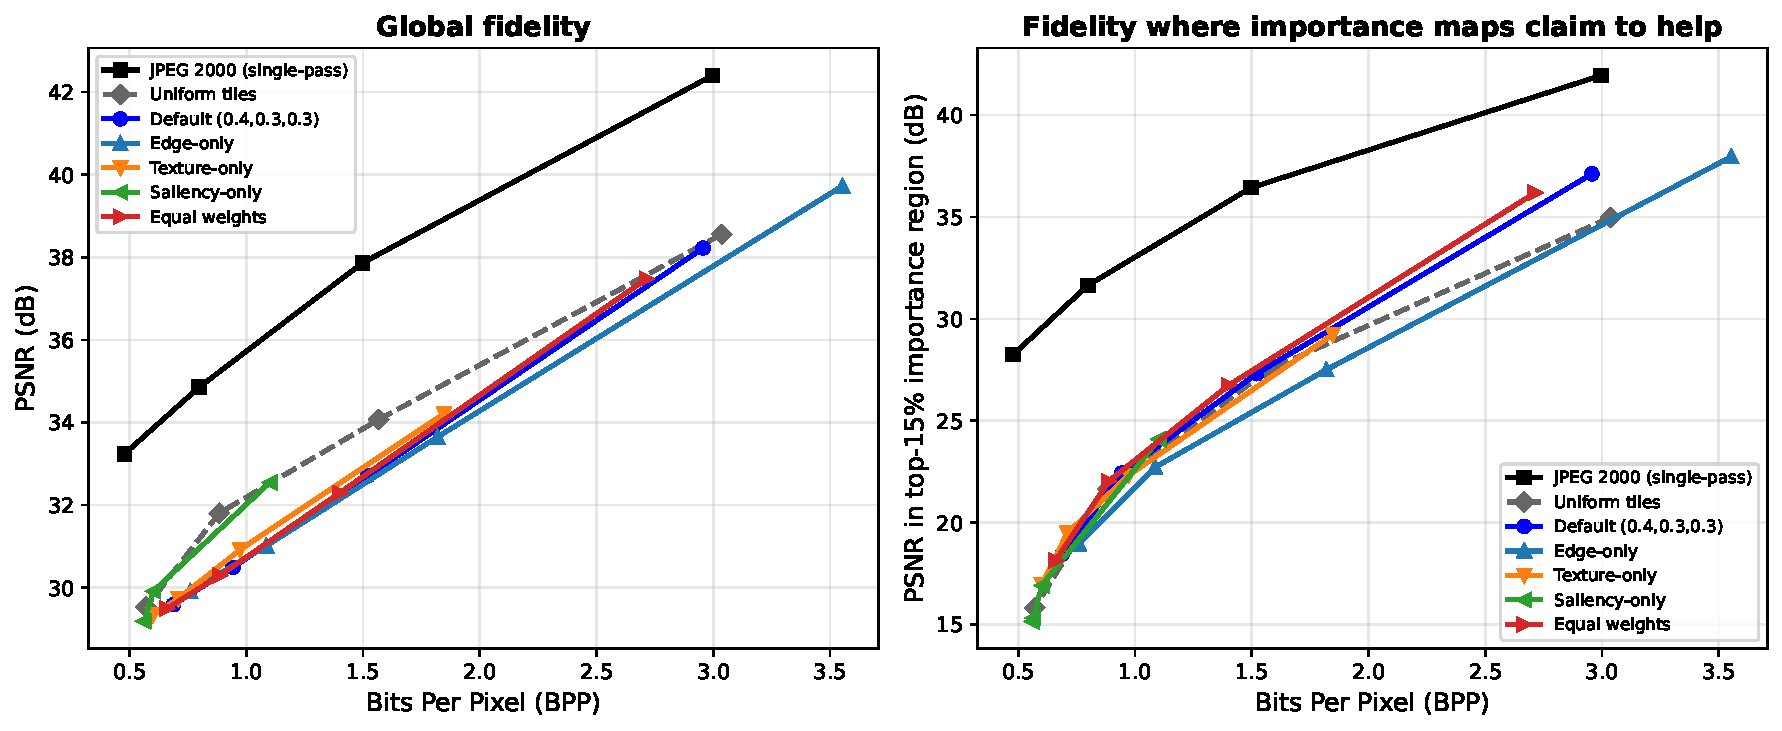
\includegraphics[width=0.92\textwidth]{figures_new/sweep_rd.pdf}
\caption{Rate--distortion on Kodak ($n{=}24$, four base ratios). Left:
global PSNR. Right: PSNR restricted to the top-15\% most-important pixels
---the regions importance maps exist to protect. Single-pass JPEG 2000
dominates every variant on both panels at every bitrate.}
\label{fig:sweep_rd}
\end{figure*}

\begin{table}[t]
\caption{Gap versus per-image single-pass JPEG 2000 anchor at matched BPP,
base ratio $R{=}16$ (mean over 24 images; all entries $p{<}0.001$).}
\label{tab:gaps}
\begin{center}
\small
\begin{tabular}{lcccc}
\toprule
\textbf{Variant} & \textbf{PSNR} & \textbf{PSNR$_{\text{hi}}$} & \textbf{PSNR$_{\text{lo}}$} & \textbf{LPIPS} \\
\midrule
Uniform tiles & $-4.00$ & $-9.23$ & $-1.34$ & $+0.04$ \\
Default & $-5.04$ & $-8.77$ & $-7.06$ & $+0.20$ \\
Edge-only & $-5.30$ & $-10.19$ & $-7.18$ & $+0.15$ \\
Texture-only & $-4.53$ & $-10.37$ & $-7.09$ & $+0.37$ \\
Saliency-only & $-3.93$ & $-12.63$ & $-7.01$ & $+0.50$ \\
Equal & $-4.95$ & $-8.64$ & $-7.06$ & $+0.22$ \\
\bottomrule
\end{tabular}
\end{center}
\end{table}

\subsection{Q1: The vehicle's cost}
The uniform row of Table~\ref{tab:gaps} isolates tile-based encoding with
\emph{no} importance signal: $-3.4$ to $-4.2$~dB globally across all four
base ratios (all $p{<}0.001$). Two mechanisms contribute: per-tile container
overhead (96 headers per image, which dominates at low rates---at $R{=}50$
the uniform-tile file is 19\% \emph{larger} than single-pass yet 4.2~dB
worse) and the loss of cross-tile redundancy and global PCRD-opt
allocation.

\subsection{Q2: Do the maps redirect fidelity as claimed? Yes---at a price}
Comparing default against uniform tiling (both anchored at matched BPP), the
importance map improves salient-region PSNR by $+3.68$~dB at $R{=}8$
($p{<}10^{-4}$) and $+1.52$~dB at $R{=}50$ ($p{<}10^{-4}$), with
non-significant gains at intermediate rates. The mechanism the literature
relies on is therefore \emph{real}. But its price is visible in the
PSNR$_{\text{lo}}$ column: the default map gives up $1.2$--$6.8$~dB of
background fidelity relative to uniform tiling for those gains---an
unfavorable exchange, and one the surveyed papers never report.

\subsection{Q3: Is the net effect ever positive? No}
Every importance variant is inferior to single-pass JPEG 2000 on every
metric at every bitrate---\emph{including inside the top-15\% regions the
maps prioritize} ($-3.3$ to $-14.0$~dB, all $p{<}0.001$;
Fig.~\ref{fig:sweep_rd}, right panel). LPIPS agrees with PSNR: all variants
are perceptually worse than single-pass ($+0.03$ to $+0.57$). The redirect
of Q2 never compensates for the vehicle cost of Q1. The sanity controls
behave as required: per-pixel random and inverted maps produce tile means
concentrated in a single ratio branch and yield output byte-identical to a
constant map (verified empirically)---so any deviation from uniform-tile
behavior is attributable to content-correlated structure, and when that
structure is present it makes results \emph{worse}, not better.

\begin{figure}[t]
\centering
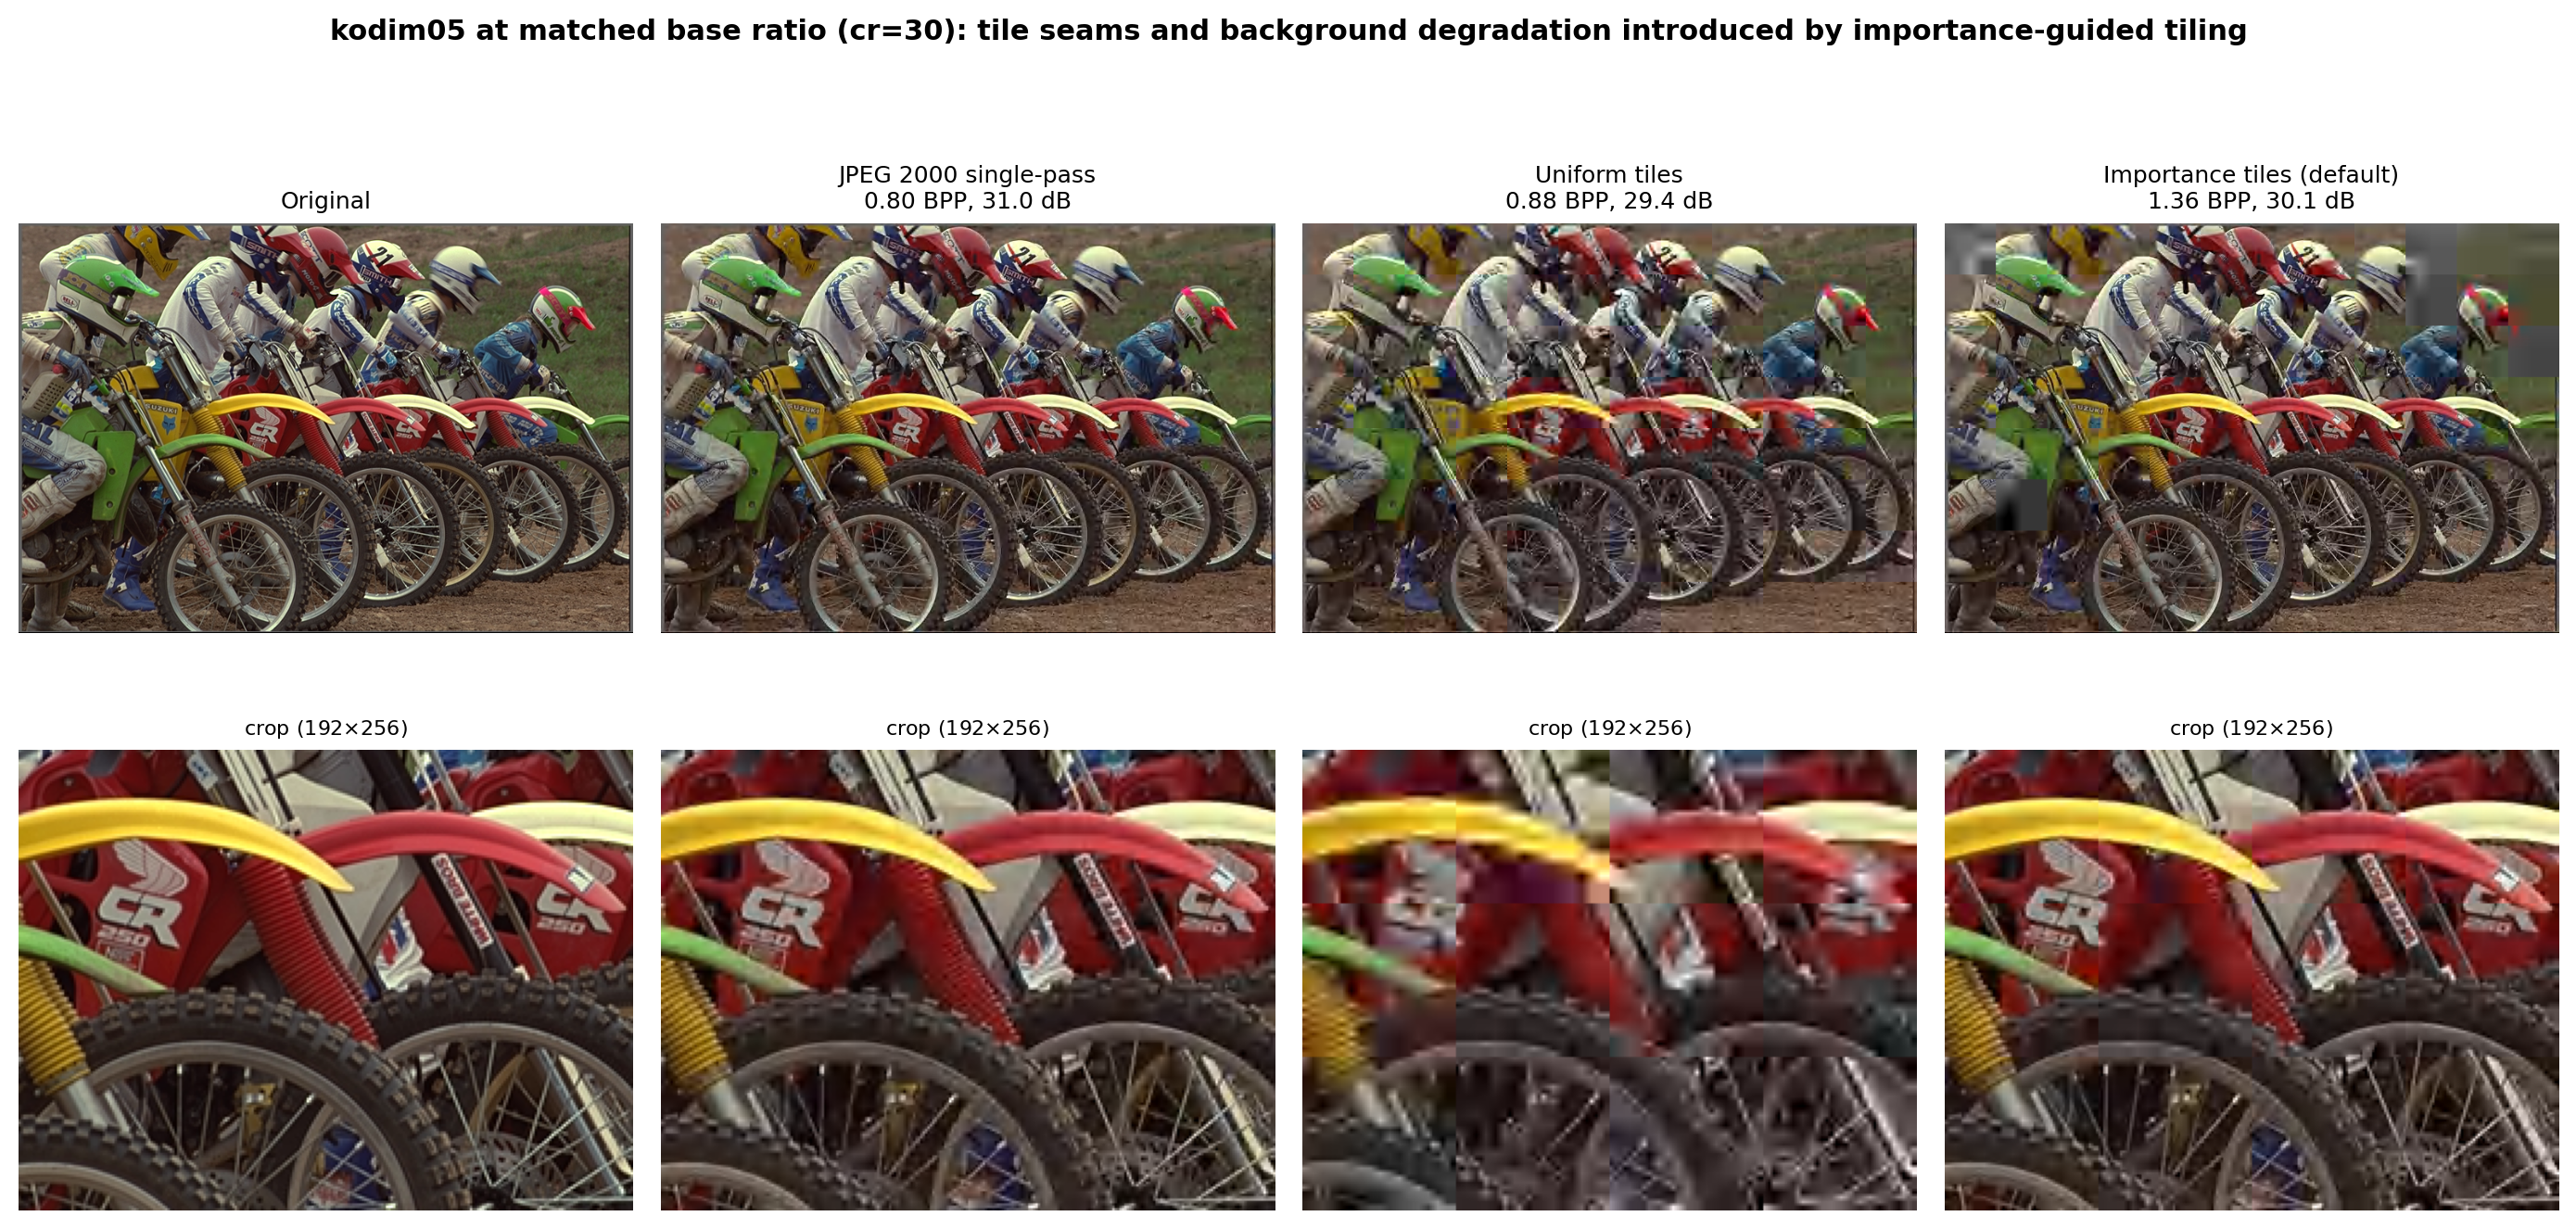
\includegraphics[width=\columnwidth]{figures_new/qualitative.pdf}
\caption{kodim05 at base ratio 30. The importance-tiled result (right) uses
71\% more bits than single-pass (left-center) yet exhibits visible tile
seams and degraded background.}
\label{fig:qualitative}
\end{figure}

\subsection{Computational cost}
Generating the three-component map takes 24.3~s per $768{\times}512$ image
(CPU), versus 0.22~s for single-pass JPEG 2000 encoding---a $110\times$
overhead for a quality reduction.

\section{Discussion}

\textbf{Why the result was predictable in one metric and not the others.}
PCRD-opt already minimizes MSE at the target rate, so \emph{global} PSNR
could not improve---our contribution there is measuring the penalty's size,
not its sign. But the literature's actual claim concerns \emph{regional}
quality, and there the outcome was open: importance maps might have won
inside salient regions. They do beat uniform tiling there (Q2), yet still
lose to the untouched codec (Q3), because the tiling machinery required to
express spatial preferences externally costs more than the preferences
recover. The implication is architectural: spatial priorities must enter
\emph{through} the codec's rate-control (Maxshift, quality-layer, or learned
rate allocation), never as an external override.

\textbf{When might external importance still pay?} Only where the vehicle is
free: codecs whose bitstream natively supports regional rates (HEVC delta-QP,
JPEG~2000 precinct/Maxshift), or learned codecs with spatially adaptive
entropy models. Our results say nothing against those designs; they say the
popular ``compute a saliency map, split the image, vary the quality''
recipe---the recipe of most of Table~\ref{tab:survey}---is worse than doing
nothing.

\textbf{Limitations.} Single dataset (Kodak); hand-crafted 2007-era saliency
rather than modern learned saliency; tile size fixed at $64{\times}64$
(smaller tiles worsen header overhead, larger tiles blur the importance
signal---neither direction rescues the approach, but we did not sweep it);
no subjective study, with LPIPS as the perceptual proxy.

\section{Conclusion}
With the two controls the literature omits---same-codec uniform allocation
and content-uncorrelated maps---hand-crafted importance-guided JPEG 2000
compression fails on its own terms: the maps demonstrably steer fidelity
toward salient regions ($+3.7$~dB versus uniform tiling, $p{<}10^{-4}$), yet
every configuration remains $3.3$--$14$~dB behind untouched single-pass
JPEG 2000 \emph{inside those very regions}, at $110\times$ the encoding
cost. Post-hoc importance masking is not a viable path to perceptual
compression; integration with the codec's rate control is the necessary
condition future work must satisfy.

\textbf{Code and data:} \url{https://github.com/abirxgpt/pair-compression}.

\begin{thebibliography}{99}

\bibitem{guo2010visual}
C. Guo and L. Zhang, ``A novel multiresolution spatiotemporal saliency detection model and its applications in image and video compression,'' \textit{IEEE Trans. Image Process.}, vol. 19, no. 1, pp. 185--198, 2010.

\bibitem{barua2015saliency}
S. Barua, K. Mitra, and A. Veeraraghavan, ``Saliency guided wavelet compression for low-bitrate image and video coding,'' in \textit{Proc. IEEE GlobalSIP}, 2015.

\bibitem{li2011visual}
Z. Li, S. Qin, and L. Itti, ``Visual attention guided bit allocation in video compression,'' \textit{Image and Vision Computing}, vol. 29, no. 1, pp. 1--14, 2011.

\bibitem{kaur2020regional}
G. Kaur et al., ``Regional bit allocation with visual attention and distortion sensitivity,'' \textit{Multimedia Tools Appl.}, vol. 79, 2020.

\bibitem{christopoulos2000jpeg}
C. Christopoulos, J. Askel\"of, and M. Larsson, ``Efficient methods for encoding regions of interest in the upcoming JPEG2000 still image coding standard,'' \textit{IEEE Signal Process. Lett.}, vol. 7, no. 9, pp. 247--249, 2000.

\bibitem{cai2017closed}
Q. Cai et al., ``Closed-form optimization on saliency-guided image compression for HEVC-MSP,'' \textit{IEEE Trans. Multimedia}, vol. 20, no. 1, 2017.

\bibitem{ouerhani2001adaptive}
N. Ouerhani, J. Bracamonte, H. H\"ugli, M. Ansorge, and F. Pellandini, ``Adaptive color image compression based on visual attention,'' in \textit{Proc. ICIAP}, 2001, pp. 416--421.

\bibitem{prakash2017msroi}
A. Prakash, N. Moran, S. Garber, A. DiLillo, and J. Storer, ``Semantic perceptual image compression using deep convolution networks,'' in \textit{Proc. IEEE DCC}, 2017.

\bibitem{zund2013content}
F. Z\"und, Y. Pritch, A. Sorkine-Hornung, S. Mangold, and T. Gross, ``Content-aware compression using saliency-driven image retargeting,'' in \textit{Proc. IEEE ICIP}, 2013.

\bibitem{zhang2021attention}
X. Zhang and X. Wu, ``Attention-guided image compression by deep reconstruction of compressive sensed saliency skeleton,'' in \textit{Proc. IEEE/CVF CVPR}, 2021, pp. 13354--13364.

\bibitem{roiswin2023}
B. Li et al., ``ROI-based deep image compression with Swin transformers,'' arXiv:2305.07783, 2023.

\bibitem{taubman2002jpeg2000}
D. S. Taubman and M. W. Marcellin, \textit{JPEG2000: Image Compression Fundamentals, Standards and Practice}. Springer, 2002.

\bibitem{wu2017just}
J. Wu, G. Shi, and W. Lin, ``Recent advances in JND modeling,'' \textit{APSIPA Trans. Signal Inf. Process.}, 2019.

\bibitem{hou2007saliency}
X. Hou and L. Zhang, ``Saliency detection: A spectral residual approach,'' in \textit{Proc. IEEE CVPR}, 2007.

\bibitem{wang2004image}
Z. Wang, A. C. Bovik, H. R. Sheikh, and E. P. Simoncelli, ``Image quality assessment: From error visibility to structural similarity,'' \textit{IEEE Trans. Image Process.}, vol. 13, no. 4, pp. 600--612, 2004.

\bibitem{zhang2018lpips}
R. Zhang, P. Isola, A. A. Efros, E. Shechtman, and O. Wang, ``The unreasonable effectiveness of deep features as a perceptual metric,'' in \textit{Proc. IEEE CVPR}, 2018, pp. 586--595.

\end{thebibliography}

\end{document}
